\documentclass{beamer}

%Style
\mode<presentation>{
%Theme
%\usetheme{default}
%\usetheme{AnnArbor}
%\usetheme{Antibes}
%\usetheme{Bergen}
%\usetheme{Berkeley}
%\usetheme{Berlin}
%\usetheme{Boadilla}
%\usetheme{CambridgeUS}
%\usetheme{Copenhagen}
%\usetheme{Darmstadt}
%\usetheme{Dresden}
\usetheme{Frankfurt}
%\usetheme{Goettingen}
%\usetheme{Hannover}
%\usetheme{Ilmenau}
%\usetheme{JuanLesPins}
%\usetheme{Luebeck}
%\usetheme{Madrid}
%\usetheme{Malmoe}
%\usetheme{Marburg}
%\usetheme{Montpellier}
%\usetheme{PaloAlto}
%\usetheme{Pittsburgh}
%\usetheme{Rochester}
%\usetheme{Singapore}
%\usetheme{Szeged}
%\usetheme{Warsaw}

%Farb-Theme
%\usecolortheme{albatross}
%\usecolortheme{beaver}
%\usecolortheme{beetle}
%\usecolortheme{crane}
%\usecolortheme{dolphin}
%\usecolortheme{dove}
%\usecolortheme{fly}
%\usecolortheme{lily}
%\usecolortheme{orchid}
%\usecolortheme{rose}
%\usecolortheme{seagull}
%\usecolortheme{seahorse}
%\usecolortheme{whale}
%\usecolortheme{wolverine}

%\setbeamertemplate{footline} % Fußzeile entfernen
\setbeamertemplate{footline}[page number] % Fußzeile entfernen und durch Folien-Zahl ersetzen

\setbeamertemplate{navigation symbols}{} % Navigations-Symbole entfernen

}

%Packages
\usepackage[utf8]{inputenc} %deutsche Umlaute
\usepackage[ngerman]{babel} %deutsche Sprache
\usepackage{graphicx} %für Bilder
\usepackage{booktabs} %für \toprule \midrule \bottomrule in Tabellen

%Einstellungen der Präsentation
\title[Ailurus fulgens]{Börsengang von Snap}
\author{Latex Tutorial}
\institute[LT]{HTWK Leipzig}
\date{\today}

%Hier beginnt die Präsentation
\begin{document}

%Titelseite
\begin{frame}
\titlepage
\end{frame}

%Inhaltsverzeichnis
\begin{frame}

\frametitle{Inhalt}
\tableofcontents

\end{frame}

\section{Grundlagen}
\subsection{Merkmale}

\begin{frame}
\frametitle{Merkmale als Fließtext}

Kleine Pandas sind etwa 120 cm lang, davon entfallen etwa 55 bis 60 cm auf den Schwanz. Ihr Stockmaß beträgt 28 cm. Männchen erreichen ein Gewicht von rund 4,5 bis 6 kg, Weibchen ca. 4 bis 4,5 kg. Sie werden durchschnittlich neun oder zehn, in Gefangenschaft auch bis maximal sechzehn Jahre alt.\\~\\
In der Gestalt sehen sie einem Waschbären ähnlich, sind aber schlanker. Ihr Fell ist lang und weich, oberseits rötlichbraun bis kupferrot, manchmal mit einem Stich ins Gelbliche, unterseits glänzt es schwarz. Das Gesicht kann individuell gefärbt sein, es ist hauptsächlich rotbräunlich mit weißen Tränenstreifen, die Schnauze ist kurz und der Nasenspiegel nackt und pechschwarz. Der Kopf ist rundlich, die Ohren sind mittelgroß, aufgestellt und laufen spitz zu, die Augen sind sehr dunkel.
\end{frame}

\begin{frame}
\frametitle{Merkmale als Bulletpoints}
\begin{itemize}
\item 120 cm \pause
\item davon 60 cm Schwanz \pause
\item 28 cm Stockmaß \pause
\item 4 bis 6 kg Gewicht \pause
\item werden bis zu 16 Jahre 
\end{itemize}
\end{frame}


\subsection{Äußeres}

\begin{frame}
\frametitle{Äußeres in Textblöcken}
\begin{block}{Körper}
In der Gestalt sehen sie einem Waschbären ähnlich, sind aber schlanker. Ihr Fell ist lang und weich, oberseits rötlichbraun bis kupferrot, manchmal mit einem Stich ins Gelbliche, unterseits glänzt es schwarz.
\end{block}
\pause
\begin{block}{Gesicht}
Das Gesicht kann individuell gefärbt sein, es ist hauptsächlich rotbräunlich mit weißen Tränenstreifen, die Schnauze ist kurz und der Nasenspiegel nackt und pechschwarz. 
\end{block}
\pause
\begin{block}{Schwanz}
Der Schwanz ist buschig, je sechsmal abwechselnd gelblichrot und ocker verwaschen geringelt, ist aber nicht zum Greifen geeignet.
\end{block}
\end{frame}

\begin{frame}
\frametitle{Mehrere Spalten}
\begin{columns}[c] %c bedeutet vertikal zentriert
 
\column{.4\textwidth} %linke spalte
\textbf{Äußere Merkmale}
\begin{enumerate}
\item Körper
\item Gesicht
\item Schwanz
\end{enumerate}

\column{.5\textwidth} %rechte spalte
In der Gestalt sehen sie einem Waschbären ähnlich, sind aber schlanker. Ihr Fell ist lang und weich, oberseits rötlichbraun bis kupferrot, manchmal mit einem Stich ins Gelbliche, unterseits glänzt es schwarz.
 
\end{columns}
\end{frame}

\section{Statistik}

\begin{frame}
\frametitle{Tabelle}
\begin{table}
\begin{tabular}{l l l}
\toprule
\textbf{2015} & \textbf{2016} & \textbf{2017}\\
\midrule
0.531 & 0.03262 & 0.562 \\
0.122 & 0.15681 & 0.910 \\
0.653 & 0.09271 & 0.296 \\
\bottomrule
\end{tabular}
\caption{Panda Verteilung}
\end{table}
\end{frame}

\subsection{Mathe}

\begin{frame}
\frametitle{Theorem}
\begin{theorem}[Äquivalenz von Masse und Pandas]
$P_{anda}=mc^2$
\end{theorem}
\end{frame}

\subsection{Optik}

\begin{frame}
\frametitle{Bild}
Rote Pandas sind so süß, dass ich eine ganze Präsentation über sie machen muss \cite{p1}. \pause
\begin{figure}
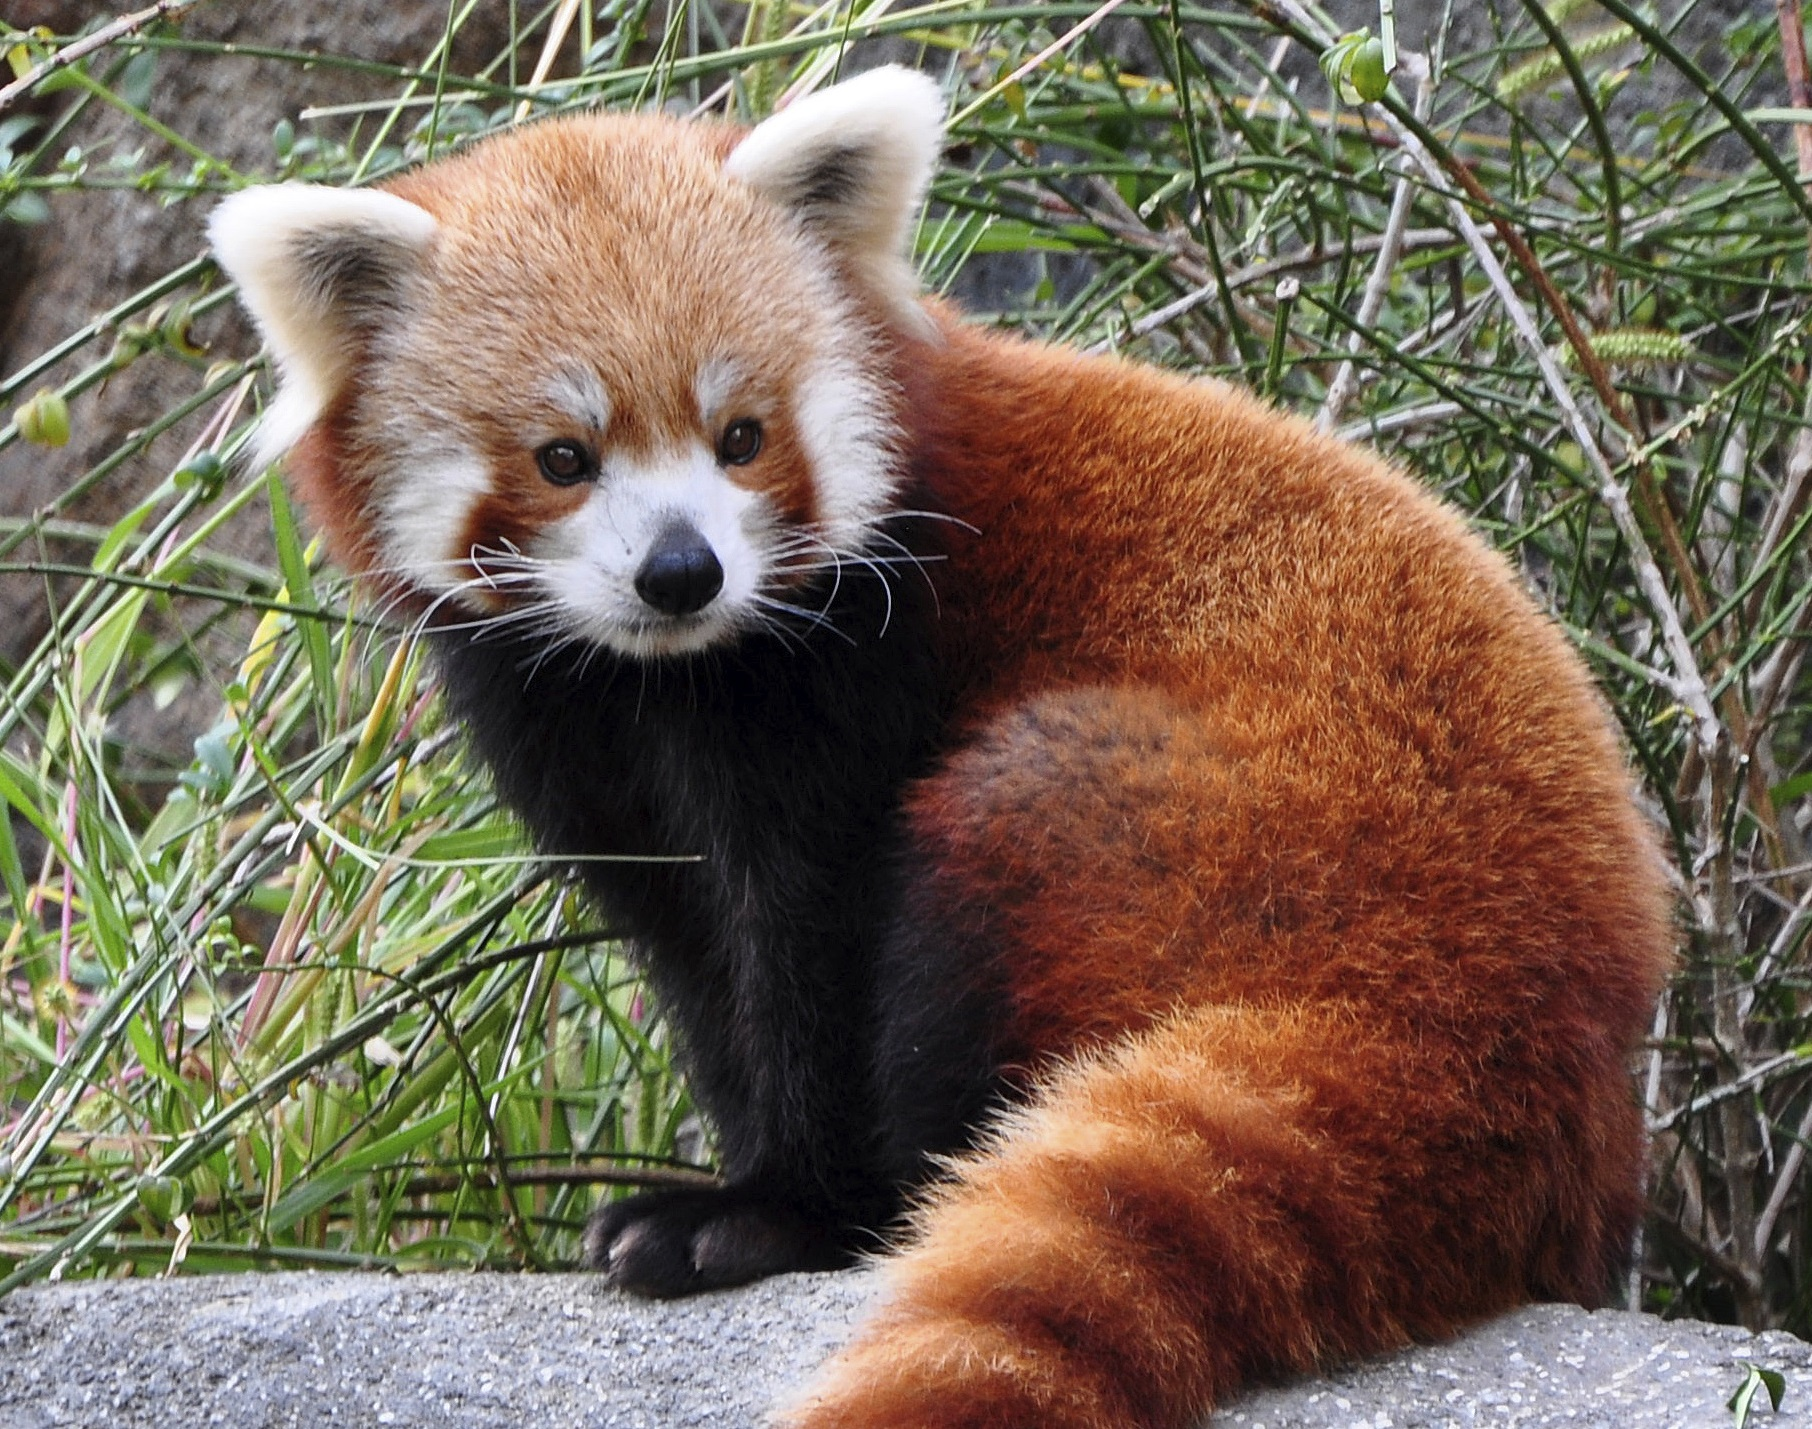
\includegraphics[width=0.7\linewidth]{panda.jpg}
\end{figure}
\end{frame}

\section{Literatur}
\begin{frame}
\frametitle{Literatur}
\footnotesize{
\begin{thebibliography}{99}
\bibitem[Wikipedia, 2017]{p1} Wikipedia (2017)
\newblock Kleiner Panda
\newblock \emph{Wikipedia{,} Die freie Enzyklopädie}
\newblock Online; Stand 24. März 2017
\end{thebibliography}
}
\end{frame}


\end{document}